\documentclass[letter]{article}
\def\baselinestretch{1.5}
\usepackage{fullpage}
\usepackage{natbib}
\usepackage{graphicx}
\usepackage{amsmath}
\author{Benjamin R. Hillman}
\title{Improving subgrid-scale clouds and precipitation in large-scale models: thesis proposal}

\begin{document}
\maketitle
\section{Introduction}
% THESIS: ambiguities in radiative fluxes and in simulated satellite-observable cloud properties from large-scale models are reduced by improving the treatment of resolved cloud and precipitation structure and overlap.

Clouds are a key piece of the global climate system, but accurate modeling of clouds in large-scale models is difficult, and cloud feedbacks in global climate models (GCMs) are recognized as a primary contributor to inter-model differences in responses to climate forcings \citep[e.g.,][]{cess_et_al_1990,bony_and_dufresne_2005,williams_and_webb_2009,medeiros_et_al_2008}.

The complexity of simulating the climate system with current computational resources limits GCM resolutions to tens or hundreds of kilometers, but clouds occur and vary on much smaller spatial scales. This means that traditional GCMs are unable to resolve individual clouds, and instead descriptions of clouds in GCMs are limited to large-scale statistical summaries of cloud properties on the scale of the model grid \citep{randall_et_al_2003}. But radiative fluxes depend on cloud properties in a non-linear manner and so the details of the unresolved structure and variability of clouds is important for model radiative transfer parameterizations \citep[e.g.,][]{barker_et_al_1999}. Most GCMs however, fail to completely account for unresolved cloud structure and variability in a sufficient manner.

% THESIS
The goal of this project is to reduce errors in radiative fluxes and simulated satellite-observable cloud diagnostics in large-scale models by improving the treatment of unresolved clouds and precipitation. The primary metric used in this study to evaluate improvements is the performance of simulated satellite-observable cloud diagnostics from the Cloud Feedback Model Intercomparison Project (CFMIP) Observation Simulator Package (COSP; Bodas-Salcedo et al., 2011) because this allows for evaluation of the simulated clouds themselves, but in so doing errors in radiative fluxes will be reduced because nominally the cloud diagnostics and radiative transfer use the same treatment of unresolved clouds and precipitation. 
This project has four main objectives:
\begin{enumerate}
    \item Quantitative evaluation of the sensitivity of COSP diagnostics to unresolved cloud and precipitation structure and variability
    \item Quantitative evaluation of the uncertainties inherent in model to observation comparisons using COSP diagnostics
    \item Develop improved treatment of subgrid-scale cloud and precipiation overlap and variability suitable for implementation in COSP and GCMs
    \item Quantitative evaluation of the sensitivity of COSP diagnostics and associated radiative fluxes to improved treatment of subgrid-scale cloud and precipitation overlap and variability
\end{enumerate}

The following section motivates the work by providing the background and context. Further motivation is provided by the Preliminary work section, which begins to address the first objective listed above. An outline for completing the last three objectives is then presented, followed by a timeline and summary.

\section{Background}
The description of clouds in GCMs typically includes profiles of partial cloudiness (cloud area fraction by level) and the in-cloud liquid and ice cloud condensate \citep[e.g.,][]{cam3_description,cam4_description}. The gridbox mean description of clouds does not in itself specify how the clouds should be distributed horizontally and vertically within model gridboxes, and characterization of the unresolved structure depends on additional assumptions about how clouds in overlapping layers are aligned vertically and how cloud properties vary within model gridboxes.

Early radiative transfer parameterizations in large-scale models used relatively simple assumptions about how subgrid-scale overlapping cloudy layers align vertically \citep[e.g.,][]{collins_2001}. These include maximum overlap, in which the cloudy portions of overlapping cloudy layers are assumed to be perfectly correlated (i.e., vertically projected cloud area is minimized); random overlap, in which the cloudy portions of overlapping cloudy layers are uncorrelated; and the popularly used maximum-random overlap, in which adjacent cloudy layers are maximimally overlapped but layers separated by at least one clear layer are randomly overlapped \citep{geleyn_and_hollingsworth_1979}. The maximal-random overlap assumption in particular has been used in a number of GCMs \citep[e.g.,][]{cam3_description,cam4_description,cam5_description}. However, these assumptions have been shown to be insufficient to capture the complexity of clouds seen in observations \citep[e.g.,][]{hogan_and_illingworth_2000,mace_and_benson-troth_2002,barker_2008}, and sensitivity tests using high resolution model simuations have shown that unrealistic overlap assumptions can lead to instantaneous errors in calculated fluxes in excess of $50 ~\text{W}/\text{m}^2$ \citep{barker_et_al_1999,wu_and_liang_2005}. \cite{oreopoulos_et_al_2012} demonstrate more modest (but still important) global mean errors on the order of $4 ~\text{W}/\text{m}^2$ in cloud radiative effects in a GCM.

Subgrid-scale variability in cloud condensate is often completely neglected in GCMs, despite the fact that clouds can exhibit large variability on scales much smaller than GCM gridboxes \citep[e.g.,][]{stephens_and_platt_1987}. This is problematic because radiative fluxes and heating rates calculated from model radiative transfer parameterizations are sensitive to subgrid-scale variations in cloud condensate \citep[e.g.,][]{barker_et_al_1999,wu_and_liang_2005,oreopoulos_et_al_2012}. \cite{barker_et_al_1999} demonstrate instantaneous flux errors due to unresolved horizontal cloud variability in excess of $100 ~\text{W}/\text{m}^2$, and \cite{oreopoulos_et_al_2012} demonstrate global cloud radiative effect errors on the order of $5 ~\text{W}/\text{m}^2$, with much larger regional errors. The sensitivity to both cloud overlap and condensate variability emphasizes the need to provide descriptions of clouds in large-scale models radiative calculations that include both horizontal variability in cloud properties and more realistic cloud overlap.

One way to account for subgrid-scale variations in cloud structure and condensate amount is to actually generate ensembles of subcolumns from the gridbox mean properties and calculate the radiative fluxes and heating rates on each generated subcolumn independently using the independent column approximation \citep[ICA;][]{cahalan_et_al_1994}. This can become computationally demanding due to the need to integrate radiative transfer calculations over a large number of spectral intervals for each subcolumn, but \cite{pincus_et_al_2003} introduced an approach that reduces the computational burden substantially by stochastically sampling both cloud state and spectral interval simultaneously. This approach, known as the Monte Carlo Independent Column Approximation (McICA), allows for fast ICA-like radiative transfer calculations (at the cost of artifically increased random noise) that can treat inhomogeneous clouds and has been incorporated into the widely used RRTMG radiation package and used in a number of state-of-the-art models \citep{iacono_et_al_2008,von_salzen_et_al_2012,cam4_description,cam5_description,donner_et_al_2011,navgem_description},

McICA separates the treatment of cloud structure and variability from radiative transfer parameterization, leaving the task of describing complex cloud structure and variability up to subcolumn sampling schemes. In principle, arbitrarily complex cloud geometries and condensate distributions can be generated by incorporating more sophisticated subcolumn schemes. However, the subcolumn schemes currently used in most GCMs make many of the same simplifications used by earlier models, including maximum-random overlap and homogeneous cloud properties \citep[e.g.,][]{cam4_description,cam5_description}. Improved subcolumn schemes are needed to take full advantage of the flexibility offered by McICA.

Unresolved cloud structure and condensate variability is important not only for calculations of radiative fluxes, but also for cloud diagnostics commonly used for evaluation of model cloud properties themselves. Satellite instrument simulators such as those provided by the CFMIP Observational Simulator Package \citep[COSP;][]{bodas-salcedo_et_al_2011} are often used to remove ambiguities in model evaluation studies that arise from uncertainties and limitations in satellite retrievals of cloud properties by producing psuedo-observations from the model state that are more directly comparable to the satellite observations \citep[e.g.,][]{klein_and_jakob_1999,webb_et_al_2001,zhang_et_al_2005,zhang_et_al_2010,kay_et_al_2012,klein_et_al_2013}. A key first step in simulating satellite observations from GCM cloud properties is accounting for the mismatch in resolved scales between the satellite pixel and model resolution by downscaling the gridbox mean cloud properties. This is done in COSP by stochastically generating subcolumns consistent with an overlap assumption to account for correlations in overlapping cloudy layers in the same manner as described for McICA above. However, the current implementation of COSP allows for only the simple maximum, random, or maximum-random overlap, and treats subcolumn clouds and precipitation as homogeneous. Furthermore, while the subcolumn treatent in COSP is intended to account for the mismatch in resolved scales between satellite pixel and model resolutions, a specific spatial scale in terms of the number of subcolumns chosen is not defined within the COSP subcolumn treatment. Condensate variability will need to be tied to an explicit scale. Also, previous studies have shown that overlap statistics are dependent on resolution \citep[e.g.,][]{mace_and_benson-troth_2002}, and so the number of subcolumns chosen within COSP should be defined in terms of model resolution in order to correctly match scales.

To the extent that the simulated satellite-observables are sensitive to these assumptions, failing to accurately characterize the subgrid cloud structure and condensate variability potentially introduces ambiguities into satellite-model comparisons. This problem deserves a closer look to build confidence in conclusions derived from these evaluation efforts. A strategy for assessing these sensitivities and for improving the representation of subgrid scale cloud and precipitation overlap and variability is presented in the following sections.

\section{Preliminary work}

\subsection{Sensitivity of simulated satellite-observable cloud diagnostics to unresolved clouds and precipitation}
\label{cosp_sensitivity}
A straightforward analysis method is used to evaluate the sensitivity of COSP diagnostics to assumptions about subgrid-scale cloud and precipitation overlap and variability. The subcolumn sampling scheme within the COSP code can be bypassed by providing fields with resolved clouds and precipitation. Assumptions about variability and overlap can then be mimicked by modifying the resolved fields used as input to the simulators, and the differences in the outputs can be taken to represent sensitivities to the modeled assumptions.

Previous studies have used cloud resolving model simulations in a similar manner to evaluate the sensitivity of radiative fluxes and heating rates to overlap and unresolved variability \citep[e.g.,][]{barker_et_al_1999,wu_and_liang_2005}. A more comprehensive sampling of different cloud regimes is obtained for this study by using output from the Multi-scale Modeling Framework \citep[MMF;][]{khairoutdinov_and_randall_2001,randall_et_al_2003}. The MMF replaces the cloud parameterizations in a traditional GCM with a 2D cloud resolving model in each gridbox. This provides global fields with resolved subgrid structure that can be passed directly to the individual instrument simulators within COSP.

In order to separately evaluate the sensitivity to overlap and heterogeneity, the following sets of modified fields are performed:
\begin{itemize}
    \item CRM: The original CRM fields within each gridbox of the MMF are used as inputs to the individual instrument simulators in COSP.
    \item CRM-AVG: cloud mixing ratios are replaced with in-cloud averages (and precipitation mixing ratios with in-precipitation averages), but the locations of hydrometeors (both cloud and precipitation) are retained from the full CRM fields at each level (i.e., occurrence overlap is retained from the CRM).
    \item CRM-RES: cloud and precipitation mixing ratios are re-sampled (with replacement) from the full CRM fields at each level within each gridbox, but the locations of these hydrometeors and their type are retained from the full CRM fields.
    \item MRO-AVG: hydrometeor mixing ratios and cloud optical properties are first averaged to produce gridbox means, similar to what a GCM would diagnose. Subcolumns are then regenerated consistent with the commonly used maximum-random overlap assumption, and homogeneous cloud properties (the gridbox means) are assigned to the cloudy subcolumns.
\end{itemize}

\begin{figure}
\centering
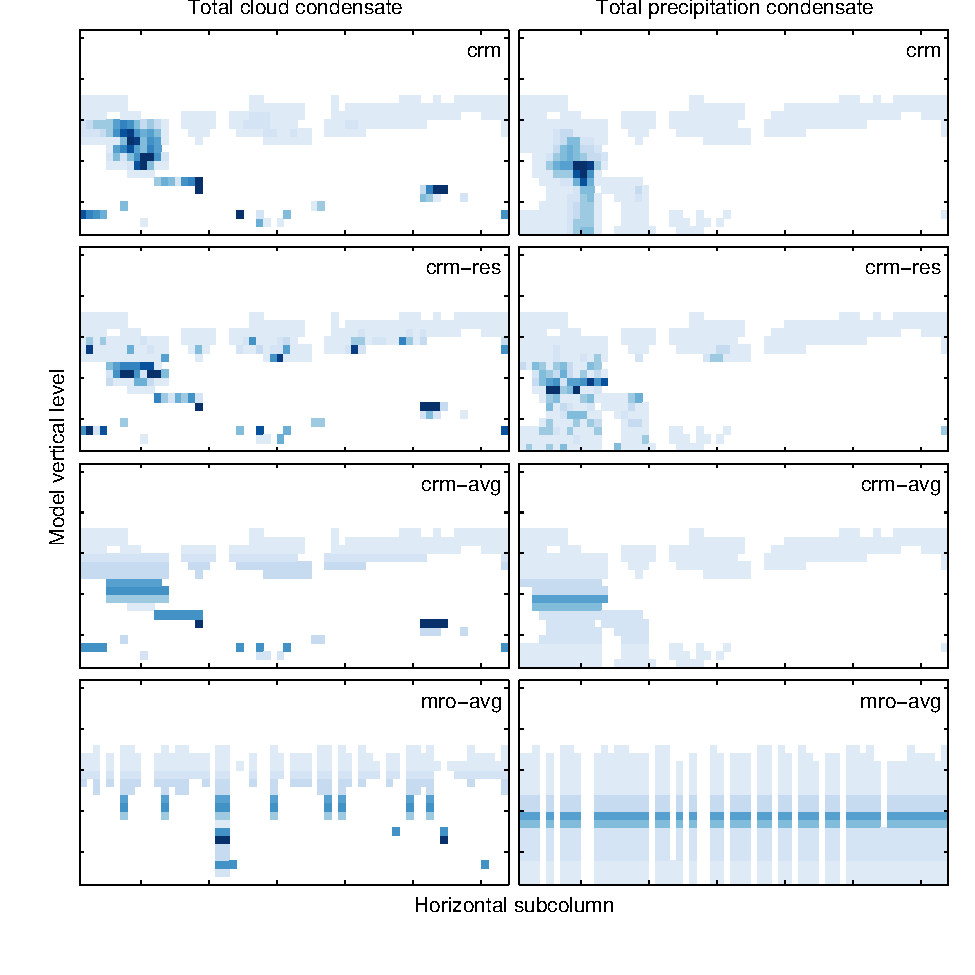
\includegraphics{test_subgrid.pdf}
\caption{Total cloud and precipitation condensate mixing ratios modified from the embedded CRM condensate mixing ratios within a single MMF gridbox.}
\label{subgrid_fields}
\end{figure}

An example of these different fields obtained from a single grid cell from the MMF is shown in Figure \ref{subgrid_fields}. The only difference between the CRM and CRM-AVG fields is that the CRM-AVG fields have homogeneous cloud and precipitation properties, so differences in COSP diagnostics calculated from these two cases represent the sensitivity to unresolved variability in cloud and precipitation properties alone. Differences between the diagnostics calculated from the CRM-AVG and MRO-AVG fields represent errors arising due to assumptions about cloud (and precipitation) overlap. The CRM-RES modification destroys any correlation between condensate amount at different levels, so differences between the CRM and CRM-RES simulations represent errors arising due to condensate amount overlap and the overlap between hydrometeor condensate of different types (clouds and precipitation).

\begin{figure}
\centering
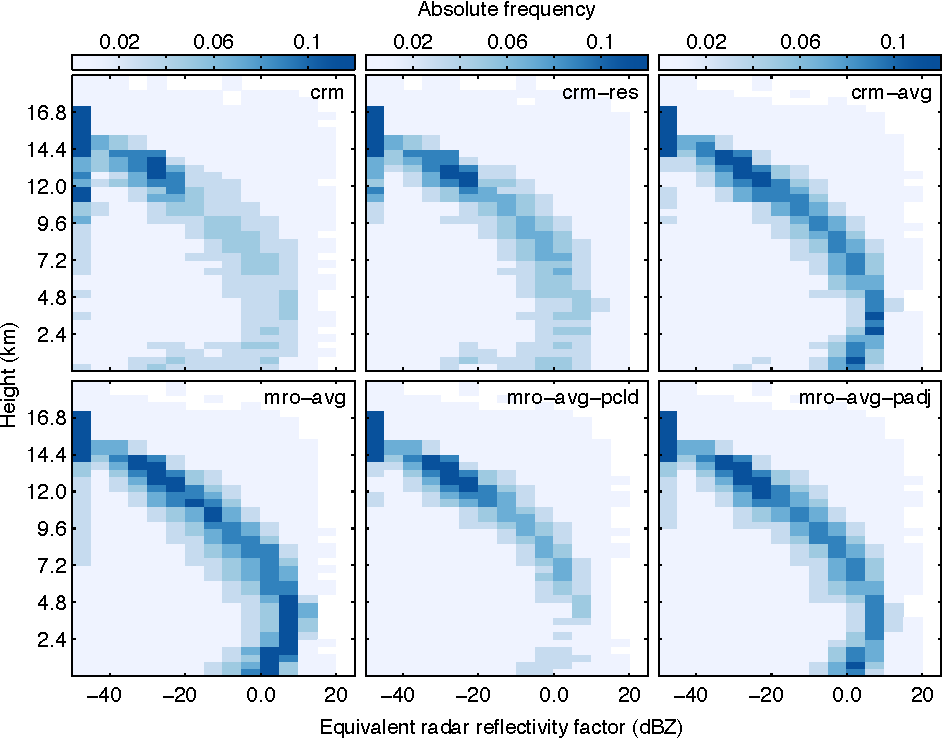
\includegraphics{radar_alt40-dbze.pdf}
\caption{Simulated CloudSat radar reflectivity factor with height histogram for the Tropical Warm Pool region.}
\label{cfadDbze94_figure}
\end{figure}


Simulated CloudSat \citep{stephens_et_al_2002} radar reflectivity factor with height histograms from these four cases are shown in Figure \ref{cfadDbze94_figure}. These histograms show a high frequency of hydrometeors along a “characteristic curve” in reflectivity-height space, with radar returns in four modes each dominated by a particular hydrometeor type \citep[described in detail by][]{marchand_et_al_2009}.

The CRM-RES simulation has more hydrometeors in middle levels above about 7 km with radar reflectivity factor between $-20$ and $10$ dBZ than the CRM simulation. Because these cases have the same level-by-level PDF of condensate amount by construction, differences between these two cases arise due to differences in the vertical alignment of condensate amount between levels. Because the CloudSat radar simulator includes the effect of attenuation of the radar signal by upper level hydrometeors, the degree to which the condensate amounts are aligned in the vertical is important. For example, if hydrometeors are aligned such that the higher condensate parts of the horizontal distributions are correlated between layers to create “pockets” of high vertically integrated water path, then there will be a greater amount of attenuation of the radar beam by the upper levels and the signal returned from the lower levels will be reduced. Since the CRM-RES simulation removes any correlation between the condensate amounts between different levels, there is less attenuation of the radar beam and more hydrometeors are apparent throughout the vertical column. The differences shown here highlight the importance of accounting for this alignment in an improved subcolumn generator. 

The CRM-AVG simulation has too many hydrometeors along the entire characteristic curve of the histogram relative to the CRM case, but this is especially evident at low levels and for radar reflectivity factor greater than $0$ dBZ. Hydrometeros in this height and reflectivity range are attributed to low-level drizzle and rain \citep{marchand_et_al_2009}, and the overestimation of hydrometeor occurrence in this mode in the CRM-AVG simulation relative to the CRM case would imply that there is too much precipitation in the CRM-AVG case. However, these cases were drawn from the same CRM simulation and by construction the precipitation fraction at each level in each large-scale gridbox (number of subcolumns containing precipitation divided by total number of subcolumns) is consistent between the two cases. This emphasizes the need to account for subgrid variability in condensate amounts (especially precipitation) in order to be able to draw correct conclusions from simulator comparisons.

\begin{figure}
\centering
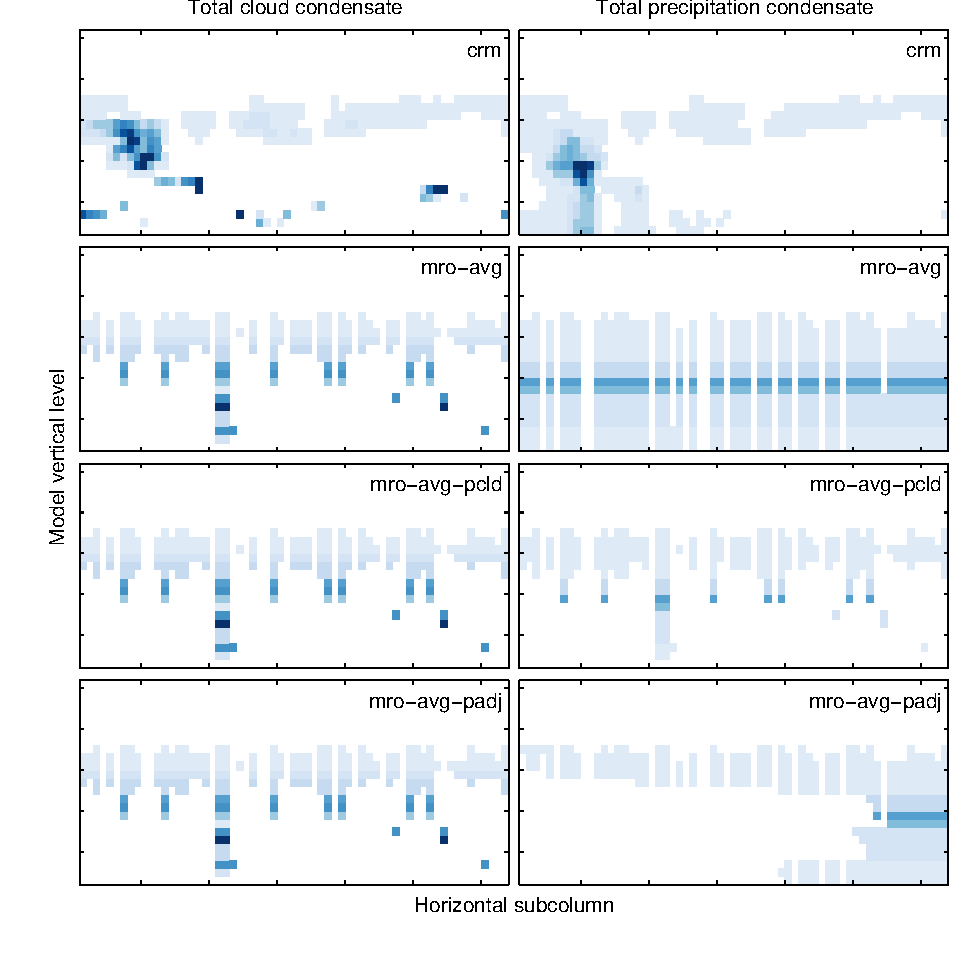
\includegraphics{test_subgrid_mro.pdf}
\caption{Total cloud and precipitation condensate mixing ratios modified from the embedded CRM condensate mixing ratios within a single MMF gridbox, showing three different methods for generating subcolumns of precipitation.}
\label{subgrid_fields_mro}
\end{figure}
The MRO-AVG simulation has even larger hydrometeor occurrence along the characteristic curve than the CRM-AVG simulation, especially for low-level hydrometeors with radar reflectivity greater than 0 dBZ. This suggests that the MRO-AVG simulation has even more widespread precipitation than the already too high CRM-AVG simulation. This is due to the simple treatment of precipitation subcolumn generation used in MRO-AVG, in which precipitation is not constrained by the actual precipitation fraction, but assigned to any level in a column in which the precipitation fraction is non-zero and contains cloud in the current column or precipitation in the column above. This likely leads to an overestimation of precipitation occurrence (suggested by the single-column example shown in Figure \ref{subgrid_fields}), and this is consistent with the overestimation of hydrometeors with large radar reflectivity factor shown here. \cite{dimichele_et_al_2012} demonstrate considerable sensitivity of simulated radar reflectivity (using a different simulator) to different approaches of generating precipitation subcolumns. The bottom panel of Figure \ref{cfadDbze94_figure} also shows results from two additional methods of treating the generation of precipitation subcolumns. The MRO-AVG-PCLD simulation restricts precipitation to only those levels within each subcolumn that contain cloud (this is the current treatment in the operational COSP code), and the MRO-AVG-PADJ simulation first distributes precipitation in the same manner as the MRO-AVG simulation described above, and then either removes or adds precipitating cells as needed to match the prescribed precipitation fraction at each level (all three methods demonstrated for a single-point example in Figure \ref{subgrid_fields_mro}). The MRO-AVG-PCLD simulation has less precipitating hydrometeors relative to the CRM and CRM-AVG simulations, consistent with the widespread removal of precipitation that results from only considering cloudy cells. The MRO-AVG-PCLD simulation appears to agree better with the full CRM simulation than the CRM-AVG simulation (which has exact overlap), but this is due to the cancellation of errors that result from too many hydrometeors along the characteristic curve due to the homogeneous condensate amounts and too few precipitating hydrometeors due to the removal of precipitation from non-cloudy levels. The adjustment of precipitating columns to match the precipitation fraction in the MRO-AVG-PADJ simulation reduces the differences relative to the full CRM simulation substantially. The sensitivity to the generation of the precipitation subcolumns demonstrated here highlight the importance of including a realistic treatment of precipitation in any subcolumn generation scheme used with the radar simulator.
%, while simulated MISR, ISCCP, and MODIS cloud top height/pressure histograms are shown in Figure \ref{cth_hist}. These results suggest that the simulated radar reflectivity is sensitive to the subgrid variability in condensate, but less sensitive to the cloud occurrence overlap, while simulated MISR, ISCCP, and MODIS histograms of CTP and cloud amount are more sensitive to both subgrid condensate variability and cloud occurrence overlap. Differences in the simulated radar reflectivity between the MRO-AVG and CRM-AVG outputs are complicated by the strong sensitivity of the radar reflectivity to precipitation, which is treated in a very simple manner in the subcolumn generator used here. Precipitation is assigned to subcolumns at levels in which the precipitation fraction is non-zero and either contain cloud at the current level or precipitation at the level directly above. As shown in Figure \ref{subgrid_fields}, this can overestimate the precipitation fraction of the regenerated subcolumns. Nonetheless, this work, along with the sensitivity of radiative fluxes and heating rates identified by others, improvements to the treatment of subgrid-scale cloud and precipitation proposed in the following section.

\begin{figure}
\centering
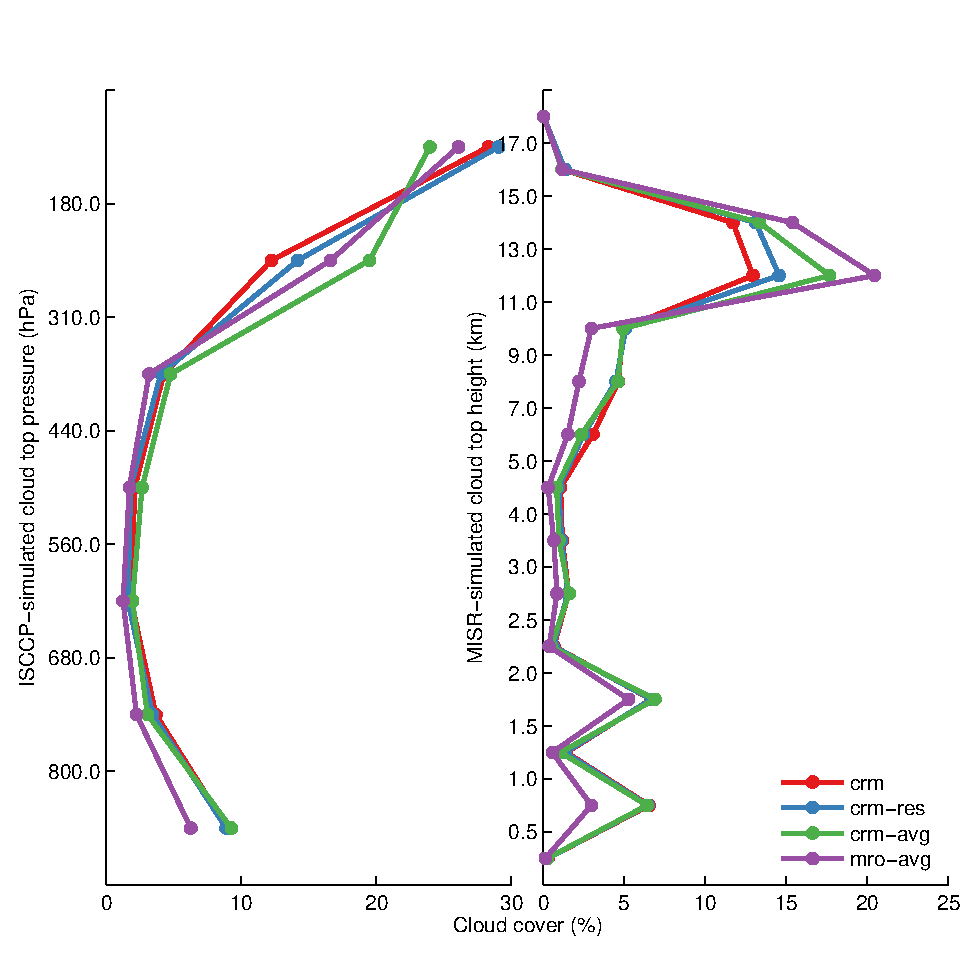
\includegraphics{isccp-misr_cth.pdf}
\caption{Simulated ISCCP cloud top pressure and MISR cloud top height histograms for the Tropical Warm Pool region.}
\label{all_cth}
\end{figure}

Figure \ref{all_cth} shows simulated ISCCP cloud top pressure and MISR cloud top height histograms for the same Tropical Warm Pool region from each of the subcolumn schemes. There are some noteworthy differences in the simulated cloud top height between the different cases, especially for the high-topped clouds. Cloud amount in the ISCCP lowest cloud top pressure bin (highest altitude) is underestimated while cloud in the second lowest cloud top pressure bin is over estimated in both cases with averaged optical properties (CRM-AVG and MRO-AVG) relative to the cases without the averaging. These differences are up to about 5\% in absolute cloud cover. The ISCCP simulator mimics the tendency for ISCCP to retrieve the radiative mean cloud top pressure in the case of multi-layer cloud profiles. If the upper layer is sufficiently thin so that a lower layer contributes to the emission seen by ISCCP, the cloud top pressure diagnosed by the ISCCP simulator will be placed lower in the atmosphere. Because the optical depth distribution is peaked sharply at low optical depth values, averaging the optical depths input to the simulator algorithm removes a good deal of the larger values that would result from variability between gridboxes, so that on average there is greater penetration of the lower-level emission that raises the retrieved cloud top pressure (lowers the cloud top height). It seems that this effect is lowered somewhat in the MRO-AVG simulation, suggesting that the maximum-random overlap assumption leads to some differences in the results as well. Others have shown \citep[e.g.,][]{mace_and_benson-troth_2002} that the maximum-random overlap can actually overestimate the vertical correlation of contiguous cloudy layers. In the case of multi-layer profiles, this could cause the upper-level cloud to appear thicker to the simulator algorithm, reducing the penetration of emission from lower levels relative to the CRM-AVG simulation. This is consistent with the results shown here.

There are much larger differences are in the MISR-simulated cloud top height, and all of the modified cases overestimate clouds with top between 11 and 15 kilometers relative to the full CRM case. The MRO-AVG has the largest departure from the CRM case, with differences approaching 10\% cloud cover and a concurrent underestimation of low-topped cloud cover. The MISR simulator mimics the tendency for the MISR retrieval to effectively see through thin upper level clouds and retrieve the cloud top height of the lower cloud layer in multi-layer profiles involving a sufficiently optically thin upper-level cloud layer and an optically thicker lower-level cloud layer. This is sensitive to the penetration depth from the top of the column at which the integrated optical depth reaches a nominal value of 1, and integrated optical depths greater than this do not further affect the assignment of cloud top height to a profile. The overestimation of clouds with cloud tops between 11 and 15 km in the CRM-AVG and MRO-AVG simulations can be explained then by the averaging of optical depths actually increasing a sufficient number of very small optical depth values so that this integrated optical depth threshold of 1 is exceeded more frequently. This seems to occur more frequently in the MRO-AVG simulation, and this can again be explained by an overestimation of the vertical correlation of vertically contiguous layers by the maximum-random overlap assumption, which results in the optical depth threshold being exceeded more frequently due to clouds lining up more than they should. This shows that both overlap and variability are important in explaining these differences, but these interpretations will need to be evaluated by examining individual single-point cases.

The differences in the ISCCP cloud top pressure and the MISR cloud top height between the different subcolumn treatments described above show that both overlap and condensate variability can affect the results of comparisons, but it is not clear from this analysis whether or not these differences are significant. A more comprehensive analysis of these differences will be included as key part of this work in order to better understand the sensitivities and uncertainties in these diagnostics. The analysis presented here will be extended to include a larger subset of regions with different cloud regimes to evaluate the importance of subgrid effects under different conditions.

It is also unclear to what extent observational uncertainty and the sensitivities of the simulators themselves (aside from subgrid effects) may affect conclusions drawn from comparisons between models and observations using these simulators. The proposed work discussed in the following section includes an analysis to quantify uncertainties in comparisons using the ISCCP and MISR simulators by comparing ISCCP and MISR data to simulated diagnostics calculated using profiles derived from observations from active profiling instruments.

The sensitivities identifed in this section motivate improvements to the treatment of subgrid variability and overlap for use in COSP.

\section{Proposed work}

\subsection{Evaluation of ISCCP and MISR simulators}
The ISCCP and MISR simulators take profiles of a model atmospheric state and attempt to determine the cloud top height and column cloud optical depth that would be retrieved by the satellite. It is assumed that if the inputs are correct, then the cloud top height and optical depth calculated by the simulator will be representative of what the satellite would retrieve. But the performance of the simulators in accurately accounting for the limitations of the satellite retrievals has not been extensively tested and documented.

\cite{mace_et_al_2010} performed a preliminary evaluation of the ISCCP simulator by using as input extinction and atmospheric profiles derived from ground-based data at the Atmospheric Radiation Measurement program (ARM) Southern Great Plains (SGP) site and comparing the simulated cloud top pressure and optical depth with collocated ISCCP retrievals. The results of their study suggest that the ISCCP simulator brings the diagnosed cloud top pressure from ARM measurements closer to those retrieved from ISCCP, indicating that the simulator reasonably accounted for features in the ISCCP retrieval of cloud top pressure. However, differences between the ISCCP-retrieved and ISCCP-simulated cloud top pressure remained unaccounted for, and the simulator fails to account for biases in ISCCP-retrieved cloud optical depths. 

While the \cite{mace_et_al_2010} study provides a first-step toward identifying ambiguities in the simulator forward operators, the results are limited to a single geographic site (which severely limits the meteorology and cloud regimes sampled), and only evaluates the performance of the ISCCP simulator. Remaining differences between the simulated and retrieved ISCCP cloud top pressure also suggest that more work should be done to understand the uncertainties in these comparisons, and in simulated diagnostics from the MISR and MODIS simulators as well. A similar analysis technique will be employed here to evaluate the performance and sensitivity of the ISCCP and MISR simulator over a larger geographic region, and to evaluate multi-layer statistics such as those described in \cite{marchand_et_al_2010} and \cite{marchand_and_ackerman_2010}.

An evaluation of the simulators over a broader geographic region and a greater diversity of cloud regimes is proposed. Extending the analysis technique used by \cite{mace_et_al_2010} is dependent on being able to obtain the needed inputs with high confidence, which include profiles of extinction, temperature, relative humidity, and visible and infrared radiances. Satellite measurements are an attractive option for the source of these inputs because they provide data with large spatial coverage, enabling an evaluation across a large diversity of cloud regimes in different geographic regions. The CloudSat cloud profiling radar \citep{stephens_et_al_2002} and the CALIPSO lidar \citep{winker_et_al_2007} have proven to be capable of accurately retrieving profiles of hydrometeor layers \cite{mace_et_al_2009}, and \cite{mace_and_wrenn_2013} describe a method for deriving extinction profiles from a combination of observations from CloudSat, CALIPSO, and MODIS. Temperature and relative humidity profiles are taken from ECMWF reanalysis mapped to the CloudSat orbit and height bins. \cite{mace_and_wrenn_2013} use these as inputs to the ISCCP simulator in order to characterize the different types of hydrometeor profiles that can be categorized into the different ISCCP CTP-OD histogram bins. But these profiles also allow evaluation of the ISCCP simulator against ISCCP observations, and the analysis can be naturally extended to include the MISR simulator and observations.

While deriving the inputs to the simulators from other satellite data enables an evaluation over a larger geographic range, it also introduces other challenges: 
\begin{enumerate}
\item Because the satellites from which the inputs are the derived and the satellites for which simulated-observations are to be evaluated are in different orbits, it is impossible to compare the simulated observations directly for each individual profile. Instead, only aggregated statistics (over a given region and time period) will be comparable. 

\item Uncertainties are introduced into the analysis by using satellite-retrieved cloud properties. CloudSat and CALIPSO are able to characterize the structure of hydrometeor layers accurately, but microphysical retrievals from radar reflectivity measurements can carry large uncertainties due to the presence of precipitation. 

\item The \cite{mace_and_wrenn_2013} retrieval uses MODIS column optical depths to constrain the extinction profiles. But the MODIS optical depth retrieval is known to be biased due to the limitations of 1D radiative transfer and the sampling restrictions of the MODIS retreival \citep{pincus_et_al_2012}. Because MISR uses a similar optical depth retrieval that is also limited by 1D radiative transfer \citep{marchand_et_al_2010}, the optical depth will likely be similarly biased, and any significant differences will likely be due to the sampling issues with the MODIS clear-sky restoral. This limits the evaluation to the simulation of cloud top height.
\end{enumerate}

After deriving the extinction profiles, the analysis technique is straightforward. The derived profiles will be used as inputs to the MISR and ISCCP simulators along with thermodynamic profiles from ECMWF reanalysis mapped to the CloudSat orbit. Cloud top height output from the simulators will be aggregated for selected regions and time periods and compared to similarly aggregated MISR and ISCCP observations. The differences will be compared against the sampling uncertainties and the uncertainties arising from the two different retrieval techniques to determine where differences are significant. In order to further evaluate the uncertainties in the simulators, the thresholds used within the MISR simulator that determine where MISR is able to see through thin cloud layers will be adjusted within reasonable values and the differences in the outputs compared against the sampling uncertainties as well to determine the sensitivity to these choices.


\subsection{Improving treatment of cloud and precipitation overlap and subgrid scale variability}
\cite{raisanen_et_al_2004} present the details of a scheme that can generate cloudy subcolumns with more flexible occurrence overlap than the commonly used maximum-random overlap and with variable in-cloud condensate for use with McICA. This scheme can serve as a starting point for developing a more complete treatment of both cloud and precipitation variability and overlap for use within COSP. %Their scheme allows for ``generalized'' cloud overlap, in which overlap is treated as a weighted combination of maximum and random \citep[e.g.,][]{hogan_and_illingworth_2000}, and has been demonstrated to better fit both observations and high resolution model simulations than simple maximum-random overlap \citep{hogan_and_illingworth_2000,mace_and_benson-troth_2002,pincus_et_al_2005,barker_2008}. Their method also allows for variable in-cloud condensate for subcolumns from an assumed probability distribution function (PDF) with prescribed vertical correlation in condensate amount.

The \cite{raisanen_et_al_2004} scheme generates subcolumn binary cloud profiles by generating real variables $x_{j,k}$ on the interval $[0,1]$ at each subcolumn $j$ and level $k$, from which the binary cloud ``fraction'' $b_{j,k}$ at each level is diagnosed by comparing $x_{j,k}$ to the partial cloudiness $C_k$ at each level, so that
\begin{gather}
    b_{j,k} = 
        \begin{cases}
            0 & \text{for } x_{j,k} \le 1 - C_k ~\text{(clear)}, \\
            1 & \text{for } x_{j,k} > 1 - C_k ~\text{(cloudy)}.
        \end{cases}
\end{gather}
To generate subcolumns with heterogeneous cloud condensate, at each subcolumn $j$ and level $k$ the cloud water content $w_{j,k}$ is assigned by generating variables $y_{j,k}$ on the interval $[0,1]$, which is then used to select the cloud water content by selecting the value $w_{j,k}$ from the normalized PDF of cloud water $p_k(w)$ that satisfies
\begin{gather}
    y_{j,k} = \int_0^{w_j,k} p_k(w)~dw.
\end{gather}
The manner in which $x_{j,k}$ and $y_{j,k}$ are chosen determines the cloud occurrence overlap (vertical correlation of the occurrence of cloud in overlapping layers) and condensate amount overlap (correlation of similar condensate magnitudes in overlapping layers). For example, allowing $x_{j,k}$ to be uniformly distributed random variables on the interval $[0,1]$ results in randomly overlapped cloud layers, and allowing $y_{j,k}$ to be uniformly distributed random variables on the interval $[0,1]$ results in heterogeneous condensate with zero correlation between levels. 

\cite{hogan_and_illingworth_2000} suggest that overlap can be well approximated by a weighted combination of maximum and random overlap, such that 
\begin{gather}
    C_{\rm gen} = \alpha C_{\rm max} + (1 - \alpha) C_{\rm ran}
    \label{generalized_overlap}
\end{gather}
where $C_{\rm max} = \max(c_k,c_l)$ is the vertically projected cloud cover assuming maximal overlap due to two overlapping layers $k,l$ with partial cloud fractions $c_k,c_l$, $C_{\rm ran} = c_k + c_l - c_k c_l$ is the vertically projected cloud cover assuming random overlap due to two overlapped layers, and $\alpha$ is the overlap parameter that determines the weighting between maximal and random overlap. \cite{hogan_and_illingworth_2000} further suggest that $\alpha$ can be approximated as a decaying exponential function of the separation distance $\Delta z = z_k - z_l$ between two layers with a decorrelation ($e$-folding) length scale of $z_{\alpha}$, such that
\begin{gather}
    \alpha(\Delta z) = \exp\left(-\frac{\Delta z}{z_{\alpha}}\right)
    \label{alpha_z}
\end{gather}
Specifying $z_{\alpha}$ then determines the overlap between pairs of layers separated by any distance $\Delta z$. In order to apply the above to their subcolumn generator, \cite{raisanen_et_al_2004} make the simplification that it is acceptable to consider only the overlap between successive adjacent layers and not between distant layers. With this simplification, their technique for generating $x_{j,k}$ for generalized overlap is as follows. First, three sets of uniformly distributed random numbers $\text{R1}_{j},\text{R2}_{j,k},\text{R3}_{j,k}$ on the interval $[0,1]$ are generated for all subcolumns $j$ and all levels $k$. $x_{j,1}$ at the top of each subcolumn is set as $x_{j,1} = \text{R1}_{j}$. Then, for each subsequent level $k$ from the second layer from the top of the atmosphere down to surface,
\begin{gather}
    x_{j,k} = \begin{cases}
        x_{j,k-1} & ~\text{for}~\text{R2}_{j,k} \le \alpha_{k-1,k} \\
        \text{R3}_{j,k} & ~\text{for}~\text{R2}_{j,k} > \alpha_{k-1,k}
    \end{cases}
\end{gather}

For heterogeneous hydrometeor fields, it has been suggested that the condensate overlap can be formulated in terms of a rank correlation $r$ between layers that specifies the degree to which the condensate amounts of similar magnitudes in the two layers are lined up \citep[e.g.,][]{raisanen_et_al_2004,pincus_et_al_2005}. Assuming a similar decaying exponential dependence for $r$ on separation distance as for the cloud occurrence overlap $\alpha$,
\begin{gather}
    r(\Delta z) = \exp\left(-\frac{\Delta z}{z_r}\right)
    \label{r_z}
\end{gather}
where $z_r$ is the decorrelation length for the rank correlation for condensate between two layers separated by a distance $\Delta z$. Again assuming that this can be applied by only considering $r_{k-1,k}$ for successive adjacent layers, $y_{j,k}$ is determined as follows. First, three more random variables $\text{R4}_{j},\text{R5}_{j,k},\text{R6}_{j,k}$ on the interval $[0,1]$ are generated at each subcolumn $j$ and level $k$. For the top layer, $y_{j,1} = \text{R4}_{j}$. For each successive layer,
\begin{gather}
    y_{j,k} = \begin{cases}
        y_{j,k-1} & ~\text{for}~\text{R5}_{j,k} \le r_{k-1,k} \\
        \text{R6}_{j,k} & ~\text{for}~\text{R5}_{j,k} > r_{k-1,k}
    \end{cases}
\end{gather}

This completely describes a method for generating subcolumns of cloud with variable condensate provided that the occurrence overlap parameter $\alpha$ (or decorrelation length $z_{\alpha}$), the rank correlation $r$ for condensate amount overlap (or decorrelation length $z_{r}$), and the normalized PDF of cloud condensate can be determined. Precipitation occurrence and condensate amount overlap could be easily prescribed using the above described framework, provided both the decorrelation lengths and the normalized PDF of precipitation condensate can likewise be defined. However, this still does not account for the concurrent overlap of clouds and precipitation (i.e., the correlation between cloud and precipitation occurrence or condensate amount), and a method for treating this will need to be developed. 

One possible way of doing this might be to first diagnose the cloudy subcolumns and cloud condensate for each cloudy cell using the above described framework. The precipitation occurrence could then be diagnosed in a similar manner to that described previously in the context of the COSP sensitivity study (the MRO-AVG-PADJ simulation), and then heterogenous condensate diagnosed via the rank correlation method described for cloud condensate, but perhaps with the additional constraint of correlation between cloud and precipitation condensate amounts prescribed. This adds another layer of complexity to the generator, and the details of how this might be implemented are not entirely clear yet. More work will need to be done in order to evaluate different frameworks for including precipitation into this scheme, and evaluating the sensitivity of the COSP diagnostics to these changes.

% Propose the following:
%   calculate cloud overlap parameter alpha from MMF output
%   calculate cloud overlap parameter alpha from CloudSat/CALIPSO mask
%   calculate precipitation overlap parameter beta from mmf output
%       calculate precipitation overlap parameter beta from TRMM PR?
%   calculate correlation between cloud and precipitation from mmf output?
%   determine appropriate PDF of both cloud and precipitation condensate to use
%   use Raisanen et al. 2004 scheme to generate clouds first; then calculate
%       p_{j,k} at all subcolumns and levels to determine precipitation by
%       determining correlation between cloud and precip?? How would this work?
In order to implement this framework to generate cloud and precipitation subcolumns with variable condensate within COSP, the following work will need to be done:
\begin{itemize}
    \item Determine the appropriate decorrelation length $z_{\alpha}$ for cloud occurrence overlap $\alpha$.
    \item Determine the appropriate decorrelation length $z_r$ for rank correlations between condensate distributions at different levels for both clouds and precipitation.
    \item Determine the correlation between cloud and precipitation condensate amount at a given level, and decide how to incorporate this into the subcolumn generator to constrain the distribution of precipitation mixing ratios
    \item Determine appropriate PDFs of both cloud and precipitation condensate.
\end{itemize}

A number of approaches have been used in the literature to determine decorrelation lengths for cloud occurrence, including ground-based radar observations \citep{hogan_and_illingworth_2000}, satellite-based cloud profiling radar and lidar observations \citep{barker_2008,oreopoulos_et_al_2012}, and cloud resolving model simulations \citep{raisanen_et_al_2004,pincus_et_al_2005}. \cite{pincus_et_al_2005} also use cloud resolving model simulations to determine decorrelation lengths for rank correlations in cloud condensate amount. While observational studies may be effective in deriving parameters for cloud condensate occurrence, this approach is challenged by the difficulty in separating clouds from precipitation in radar observations due to the strong sensitivity of reflectivity from cloud profiling radar to large particles. This makes deriving cloud water content from radar reflectivity measurements difficult, and because the radar signal is dominated by precipitation when precipitation is present this approach will be insufficient for characterizing the overlap between clouds and precipitation. Modelling approaches such as that performed by \cite{pincus_et_al_2005} can be useful here because they simultaneously provide estimates of both cloud and precipitation distributions from which the overlap statistics can be derived. The downside of the modelling approach is that the cloud fields used to derive the overlap parameters are not guaranteed to accurately portray clouds in nature, which makes model-derived overlap parameters approximate at best. Nonetheless, high-resolution models can be used to provide a first-guess at the overlap parameters, which can later be checked against available observations for consistency where accurate observations are available.

The approach used here will be to derive decorrelation length scales for cloud and precipitation occurrence and condensate amount overlap from model output from the MMF. This allows for an analysis of overlap parameters over a complete range of cloud and meteorological regimes. \cite{pincus_et_al_2005} describe a straightforward method for deriving overlap statistics, which will be used to study overlap in the MMF output. Combined vertically projected cloud cover $C_{\rm true}$ is calculated for pairs of layers within a specified domain at each time step and at each gridbox. The theoretical vertically projected cloud covers $C_{\rm max}$ and $C_{\rm ran}$ (defined above) are also calculated for each pair of layers, which represent the cloud cover that would be observed if the overlap were maximum or random, respectively. The overlap parameter $\alpha$ is then calculated for each pair of layers by solving Equation \ref{generalized_overlap} with $C_{\rm gen}$ replaced with $C_{\rm true}$. This can be done using the instantaneous vertically projected cloud covers and then taking the time average of $\alpha$, or the time averaged cloud covers can be calculated first and an average $\alpha$ calculated using the time averaged cloud covers. In either case, $\alpha$ is then plotted against layer separation $\Delta z$ and fit with an exponential with the form of Equation \ref{alpha_z} to obtain an estimate of the decorrelation length $z_{\alpha}$. This will be done for both clouds and precipitation.

The decorrelation length for rank correlations between layers is calculated by first calculating the rank of the distribution of condensate at each layer within each gridbox, defined such that the column with the smallest mixing ratio in a given layer has rank 1, the column with the next smallest mixing ratio has rank 2, and so forth. The rank correlation $r_{k,l}$ between layers $k,l$ is then just the spatial correlation of the rank for each pair of layers. The rank correlation is then plotted against layer separation and fitted with an exponential with the form of Equation \ref{r_z}. This is done separately for both clouds and precipation.

\cite{mace_and_benson-troth_2002} and \cite{barker_2008} show that the decorrelation length for cloud occurrence overlap calculated similarly to that described here varies with geographic location, season, and resolution. Rather than deriving a set of decorrelation lengths specific to location and season explicitly as done in \cite{oreopoulos_et_al_2012} (which would not be guaranteed to hold under all conditions or in a changing climate), decorrelation lengths will be parameterized in terms of the atmospheric state by exploring the dependence of decorrelation lengths on different model fields. It is not entirely clear on what the overlap parameters should depend, but \cite{pincus_et_al_2005} suggest a dependence on wind shear and convective strength as a good starting point. This is intuitive, because wind shear can be expected to decrease organization between layers while convective activity should tend to increase organization between layers (by making cloud more verically contiguous). The dependence of cloud and precipitation overlap decorrelation lengths on these fields will be evaluated as a starting point.

In order to characterize the condensate overlap between clouds and precipitation, the rank of cloud water content and the rank of precipitation water content can be calculated separately at each level within each gridbox of the MMF, and the spatial correlation between the cloud and precipitation ranks calculated to determine the degree to which the distributions of cloud and precipitation mixing ratios are lined up. This analysis will help determine how to distribute variable precipitation condensate to appropriately line up with cloud condensate as distributed via the \cite{raisanen_et_al_2004} method described.

The PDFs of cloud and precipitation condensate mixing ratios still need to be determined in order to generate subcolumns with the appropriate subgrid variability. Again, satellite retrievals of condensate mixing ratios are problematic due to the ambiguities in separating clouds from precipitation, and case studies using aircraft observations are limited in sampling.  An analysis of MMF output will be used to get an estimate of the variability in condensate mixing ratios, with the understanding that fits to the MMF output will only be approximate given the conceptual limitations of using even a sophisticated model to infer properties of the real world. This will be sufficient for this study because the purpose is not to develop a final parameterization suitable for all models, but rather to assess the sensitivity of model diagnostics to improvements in the treatment of subgrid structure and variability.

With recent interest in PDF-based cloud parameterizations \citep[e.g.,][]{tompkins_2002}, it makes sense to eventually connect the subcolumns used by the radiative transfer and COSP modules to those used in the cloud physics parameterizations directly in the context of implementation in a GCM. There is an on-going project to implement the Cloud Layers Unified By Binormals \citep[CLUBB][]{golaz_et_al_2002} into the National Center for Atmospheric Research (NCAR) Community Atmosphere Model (CAM), which would naturally provide the subgrid-scale variability in total water and rain water mixing ratios needed. Much of the work has already been done to pass PDFs of condensate from CLUBB to the radiation code in the development version of CAM5 (Andrew Gettelman, personal communication), and it would likely be straightforward to extend this to either pass the subcolumns generated by the McICA code to COSP, or to similarly pass the PDFs of condensate to an improved COSP subcolumn sampler to include the subgrid variability. This is a possible avenue for future work, but is beyond the scope of this study.

%\cite{oreopoulos_et_al_2012} test the sensitivity of a global climate model to improved subgrid clouds using the \cite{raisanen_et_al_2004} generator. They derive approximate decorrelation depths $\alpha(\Delta z)$ that vary with latitude and season from an analysis of CloudSat data, and use beta distributions to describe the variability of in-cloud condensate. Their results show that improvements in radiative fluxes due to implementation of this scheme are important, but their simple latitude and seasonal dependence of decorrelation depths are not guaranteed to hold in a changing climate, and parameterization of these quantities in terms of model fields is probably a better approach for operational use in a model intended to aid understanding of the climate system in response to changes. \cite{pincus_et_al_2005} derive decorrelation depths from cloud resolving model data, and suggest parameterizing these in terms of large-scale fields such as wind shear and convective strength. They provide such a parameterization, but limited to a single domain over the ARM SGP site. Nonetheless, this is a good start, and this is an attractive avenue for further parameterization of these quantities.


%I propose a characterization of overlap statistics using output from the MMF to add to the work already done by others, and to separately diagnose overlap of clouds and precipitation which is difficult to do using radar observations as done by \cite{hogan_and_illingworth_2000},\cite{mace_and_benson-troth_2002}, and \cite{barker_2008}. The advantage of using the MMF for these studies is that it provides a complete description of subgrid-scale clouds and precipitation across all regimes and inludes the large-scale fields available in a traditional GCM, which will likely be useful for parameterizating the overlap characteristics. The limitation with this approach is that the MMF is still a model, and may not completely capture the complexity of the real atmosphere. In order to address this issue, I also plan to use hydrometeor occurrence profiles derived from CloudSat \citep{stephens_et_al_2002} and CALIPSO \citep{winker_et_al_2007} observations to independently derive overlap statistics in a similar manner as done by \cite{barker_2008} to compare with my characterization of overlap derived from MMF output. The goal is for this analysis to result in a parameterization of decorrelation lengths for both cloud and precipitation occurrence and condensate overlap based on large-scale fields. As suggested in the previous section, treating the precipitation in a more realistic manner will be important in accurately simulating radar reflectivities.

\subsection{Sensitivity of COSP simulator diagnostics to improvements in the treatment of cloud and precipitation overlap and subgrid-scale variability}
Following the characterization of overlap statistics and subgrid-scale variability for the \cite{raisanen_et_al_2004} subcolumn generator with the extensions proposed in the previous section to include precipitation, the next step is to implement the improved scheme into COSP and test the sensitivity of the simulated satellite-observables to the improvements. 

Implementation of an improved subgrid treatment is relatively straightforward in the stand-alone COSP code, and the new subcolumn generator can just replace the ``SCOPS'' and ``PREC\_SCOPS'' modules in that code. The sensitivity of the COSP diagnostics to the improvements in the treatment of subgrid clouds and precipitation will be tested using MMF output with a similar framework as used for the baseline sensitivity tests in Section \ref{cosp_sensitivity}. COSP diagnostics will be calculated using the full CRM fields from the MMF to provide a baseline for comparison. Additional cases will be created by calculating gridbox means from the MMF CRM fields to mimic what a traditional GCM would produce, and these fields will be used to calculate COSP diagnostics which will then be compared against those calculated from the full CRM fields. 

Diagnostics will be compared at the global, zonal, and regional scales across a range of cloud and meteorological regimes in order to evaluate the sensitivies of the diagnostics to the changes in the context of common model evaluation strategies. The result of this analysis will be a quantification of the sensitivity of COSP diagnostics to changes in the treatment of subgrid cloud and precipitation overlap and variability. This will also serve as motivation for future efforts to better incorporate these effects into GCMs in the context of both satellite simulators and radiative transfer.

%Sensitivity of the COSP diagnostics will be tested alongside the radiative fluxes and heating rates in the context of the CAM5 implementation. The stand-alone COSP subcolumn scheme will be tested using MMF output and a similar framework as described above for the baseline sensitivity tests of the COSP outputs.

%For use in CAM5, however, these modules should be bypassed and common subcolumns between COSP and the McICA radiative transfer code should be used to enforce consistency between the radiative transfer and the (radiatively-important) satellite-observable cloud diagnostics. 

%As mentioned above, the infrastructure to sample subcolumns with variable condensate from CLUBB PDFs has already been implemented in the development version of the CAM5. It should then be straightforward to either pass subcolumns with subgrid variability generated for the radiation code to COSP, or to pass CLUBB PDFs of condensate to COSP for generation of the subcolumns. This will allow for concurrent evaluation of the sensitivity of both radiative fluxes and COSP diagnostics to changes in the treatment of the subgrid cloud and precipitation structure and variability, with variability specified by the CLUBB physics parameterization. It is not clear yet whether or not their implementation generates subcolumns of precipitating hydrometeors. This will be important for the COSP diagnostics, and may need to be added or improved depending on what they have done.


%Implementing generalized overlap and in-cloud variability in condensate using the \cite{raisanen_et_al_2004} method requires specification of the overlap parameter that determines the weighting between maximal and random overlap, the PDF of condensate distribution, and the rank correlation between condensate amounts in different layers. \cite{hogan_and_illingworth_2000} suggest that the overlap parameter $\alpha$ can be approximated as a decaying exponential function of separation distance $\Delta z$ between layers, such that determining $\alpha$ is akin to specify the e-folding depth $z_{\alpha}$. \cite{raisanen_et_al_2004} suggest that the rank correlation $r$ can likewise be approximated as an exponential function of separation distance between layers, with a separate e-folding depth $z_{r}$.

%After performing a baseline assessment, the next and probably most difficult step is to develop or select a parameterization of subgrid-scale cloud variability. I think the most natural way to integrate a model for subgrid-scale variability into radiative schemes used in large-scale models is to take a PDF-based approach for use with the McICA. Such a method would presumably prescribe a PDF of cloud optical properties based on the large scale atmospheric state and the grid-box mean quantities. I believe such a scheme has already been implemented to an extent in the latest climate model produced by CCCma, the CanAM4 \citep{von_salzen_et_al_2012}, which assumes a gamma distribution for the cloud condensate based on previous studies such as that by \cite{barker_1996}. I have had some preliminary conversations with Jason Cole at CCCma about this, and he is interested in expanding upon their parameterization and further discussing possibilities with us for how to do this. I'm not completely clear on the details of the current implementation, and more discussions on this need to take place.

%The aforementioned strategy may provide for a flexible implementation applicable to a range of climate models, and in particular may lend itself to development of an improved stand-alone subcolumn generator for COSP, but with recent interest in PDF-based cloud parameterizations it may make more sense to connect the subcolumns used by the radiative code to those used in the cloud physics parameterizations more directly. There is an on-going project to implement the Cloud Layers Unified By Binormals \citep[CLUBB][]{golaz_et_al_2002} into CAM, which would naturally provide the subgrid-scale variability we are after \citep{wood_2012}. Rob Wood expressed interest in discussing this further and keeping in touch on this front.

%\subsection{Implementing in a large scale model}
%The next step would be to implement the parameterization of subgrid-scale clouds into a large-scale model and to test the impact of the changes on the calculated fluxes and heating rates and the simulated cloud diagnostics. Again, I think CAM5 would make an excellent test-bed for this, since much of the machinery is already in place (McICA, and on-going development to include a PDF-based cloud scheme).

%In the case of developing a new subcolumn generator that is somewhat independent of the cloud physics parameterization (i.e., the first method described in the previous subsection, not the integrated CLUBB method), the parameterization can be tested before being implemented into a particular large-scale model. This can be done by using fields generated by a cloud resolving model, and applying various averaging methods and radiative transfer solvers. One strategy would be to take a domain maybe the size of a typical climate model grid-box for a particular case. A benchmark calculation might be to run an ICA radiative transfer code on the fully resolved CRM fields. One test might consist of averaging the CRM fields over the horizontal domain, assigning subcolumns using the new subcolumn generator, and running the ICA code on the generated subcolumns and comparing the fluxes and heating rates with the ICA calculation on the fully resolved CRM fields. This would test the parameterization of subgrid-scale clouds. A further test may be to do a McICA calculation on the generated subcolumns, and compare to the two ICA calculations.

\section{Expected outcomes and timeline}
The following outcomes are expected from this work:
\begin{itemize}
    \item Quantitative evaluation of uncertainties in model-observation comparisons using COSP diagnostics (Fall 2014)
    \item Quantitative evaluation of the sensitivity of COSP diagnostics to unresolved cloud and precipitation structure and variability (Fall 2014)
    \item Characterization of subgrid-scale cloud and precipitation structure and variability (Winter and Spring 2015)
    \item Quantitative evaluation of the sensitivity of COSP diagnostics to improved treatment of subgrid-scale cloud and precipitation overlap and variability (Spring and Summer 2015)
\end{itemize}

\section{Summary and impacts}
Subgrid-scale variability in cloud structure and cloud properties have been shown by others to affect radiative fluxes and heating rates calculated by 1D radiative transfer codes in large-scale models, and are shown in the first part of this work to affect calculations of simulated satellite-observable cloud diagnostics. The latter are commonly used to assess the fidelty of models in simulating cloud properties consistent with present day observations, and so ambiguities arising due to neglect of important subgrid structure and variability potentially weaken some of the conclusions reached with these studies. The results of the present work will improve the representation of the subgrid-scale structure and variability of clouds and precipitation, and thereby lead to improved simulation of fluxes and heating rates and simulated satellite observerable cloud diagnostics in models. The improvement in fluxes and heating rates may reduce compensating errors in cloud properties, where tuning efforts have historically been needed to adjust cloud properties away from reasonable values in order to obtain radiative balance in climate simulations. The improvement in simulated satellite-observable cloud diagnostics will reduce ambiguities and uncertainties in comparisons between modeled and observed clouds and lead to more robust model evaluation.
\bibliographystyle{ametsoc}
\bibliography{proposal}
\end{document}

%The problem of inferring smale-scale structure from the large-scale description of cloud properties is not unique to simulated satellite diagnostic quantities. Because radiative transfer depends on the cloud properties in a non-linear manner, the details of the small-scale structure and variability are critical in calculating the large-scale fluxes and heating rates \citep[e.g.,][]{wielicki_and_welch_1986,boer_and_ramanathan_1997,stubenrauch_et_al_1997}. The cloud overlap problem consequently has a long history. Early radiative transfer parameterizations in GCMs used idealized, simplistic overlap assumptions hard-coded deep within the radiative transfer code (e.g., ???), and assumed that cloud condensate was constant on the scale of GCM gridboxes (plane parallel homogeneous). Until recently a majority of models \citep[e.g.,][]{cam3_description,cam4_description,cam5_description,am2_evaluation} have used the maximum-random overlap assumption \citep{geleyn_and_hollingsworth_1979,stubenrauch_et_al_1997,collins_2001}, in which clouds in adjacent cloudy layers are assumed to be maximally overlapped (perfect correlation) and clouds in layers separated by one or more clear layers are assumed to be randomly overlapped (no correlation). However, a number of studies have shown that these simplistic assumptions of cloud overlap fail to capture the complexity of clouds in nature \citep[e.g.,][]{hogan_and_illingworth_2000,mace_and_benson-troth_2002,pincus_et_al_2005,barker_2008} and can lead to substantial biases in top of atmosphere fluxes and domain-averaged profiles of radiative heating rates \citep{barker_et_al_1999,oreopoulos_et_al_2012}. \cite{barker_et_al_1999} and \cite{oreopoulos_et_al_2012} show that the assumption of homogeneous cloud condensate amount on the scale of GCM gridboxes is also inappropriate and leads to errors in radiative fluxes and heating rates.


%Subgrid-scale variability in the liquid and ice cloud condensate amount is often neglected in large-scale models, and these quantities are typically assumed to be homogeneous in the cloudy portions of each layer in each column \citep[e.g.,][]{cam3_description,cam4_description,cam5_description,am2_evaluation,donner_et_al_2011}. Yet, cloud properties can exhibit substantial variability on scales much smaller than the resolutions typical of large-scale models (citations?). \cite{barker_et_al_1999} showed that neglecting this variability can lead to large biases in shortwave fluxes. Moreover, clouds can have more complicated vertical structure than is often represented by simple overlap assumptions (citations?), and \cite{barker_et_al_1999} show that incorrect overlap of clouds can also contribute to large biases in fluxes and heating rates. This emphasizes the need to provide more realistic descriptions of clouds as seen by the radiative transfer solvers in large-scale models that include both horizontal variability in cloud properties and more realistic cloud overlap.

% Sensitivity of simulated satellite-observables to unresolved variability and overlap
%   MMF
%   CRM-HET vs CRM-HOM: errors due to homogeneous clouds and precip
%   MRO-HOM vs CRM-HOM: errors due to max-rand overlap assumption
% Parameterizing subgrid-scale cloud structure from the large-scale means: improvements
%   McICA: stochastic sampling of cloud states
%   Include variable condensate amount in subcol generation
%   Include overlap of condensate amount
%   Include more flexible treatment of cloud overlap

%It is well-known that neglecting subgrid-scale variability in plane-parallel homogeneous radiative transfer calculations can lead to biases in computed fluxes and heating rates in large-scale models, and a number of strategies have been proposed and tried to deal with this problem. One strategy which has seen use in global climate models \citep[e.g.,][]{am2_evaluation} has been to scale cloud optical properties in some way so that the computed fluxes more closely match those observed. Different scalings have been proposed by \cite{davis_et_al_1990}, \cite{cahalan_et_al_1994}, and \cite{cairns_et_al_2000}. However, using only a single scaling with this strategy has been shown to work only for a narrow range of optical depths and solar zenith angles \citep{cahalan_et_al_1994,barker_1996}. The ideal scaling factor has also been shown to be dependent on gridbox size \citep{pomroy_and_illingworth_2000}, spectral region \citep{yu_et_al_1997}, and on geographic region \citep{oreopoulos_and_cahalan_2005}. The dependence on geographic region is particularly troubling for implementation in climate models, which are used to model the atmosphere and make predictions about climates which may differ significantly from the current climate.

%While radiative fluxes and heating rates depend critically on the description of clouds in models (including assumptions about the subgrid scale as described above), errors in the representation of cloud properties can cancel each other to produce radiative fluxes in good agreement with observations \citep[e.g.,][]{kay_et_al_2012}.  This is not too surprising, as GCM are often ``tuned'' to achieve radiative balance at the top of the atmosphere by adjusting variables within parameterizations in the models (citations?). An example of this is the commonly cited ``too few, too bright'' problem where models can produce top of atmosphere fluxes in good agreement with observations by having too little cloud cover with optical depths that are too large \citep[e.g.,][]{zhang_et_al_2005,klein_et_al_2012,nam_et_al_2012}. Because of this, it is important to evaluate the diagnosed cloud properties themselves, and a great deal of effort has been put into evaluating cloud properties in simulations of present day climate against available observations as a test of their validity \citep[e.g.,][]{gleckler_et_al_2008,zhang_et_al_2005,kay_et_al_2012,klein_et_a_2013} (others?). 

%Satellite observations of cloud properties can be useful as a baseline for comparison because they provide near global coverage, but comparisons of this sort can be challenging due to the fact that the quantities measurable from space are quite different from those that can be simulated by models. While models can diagnose relevant geophysical quantities directly (e.g., cloud fraction, cloud height, cloud liquid and ice water content, particle size), satellites must infer these quantities from measured radiances using inversion techniques (retrieval algorithms; cite examples). Cloud properties retrieved by these techniques can often carry large uncertainties due to the challenges and limitations of the instruments and inversions \citep[e.g.,][]{marchand_et_al_2010,pincus_et_al_2012} (others?).

%\cite{barker_1996} and \cite{oreopoulos_and_barker_1999} proposed other approaches to treat the subgrid heterogeneity which involved weighting the optical depths used in the radiative transfer equations by a distribution function. Their particular method has been referred to as the ``gamma-weighted two-stream approximation.'' \cite{oreopoulos_and_barker_1999} implemented this scheme in a large-scale model and were able to reduce plane-parallel-homogeneous biases relative to 3D Monte Carlo and ICA calculations, but with increased computational cost (a factor of two or greater).

%\cite{shonk_and_hogan_2008} proposed a method in which each vertical level in the model is broken into three regions: one for the clear-sky portion of each grid-box, one for the optically thin clouds and one for optically thick clouds in each grid-box. A probability distribution for cloud water is modelled or assumed, and selecting a value representing the lower percentile and a value representing the upper percentile of the distribution defines the two cloudy regions in each level. Selecting different percentiles has the effect of varying the amount of variability represented. This method has the advantage of being computationally efficient and has the potential to reduce plane-parallel biases by providing more information about the distribution of cloud water in a grid box (two values instead of one), but the full distribution of cloud water is not sampled. Also, to implement this scheme in a model would require modifications to the radiation code itself in order to handle the two cloudy regions in each level. Also, this may not extend naturally to implementation in subcolumn sampling codes used in instrument simulator diagnostics \citep{klein_and_jakob_1999}.

%Perhaps the most straightforward and accurate way to account for subgrid-scale variability in cloud structure and properties would be to assume some probability distribution for each grid-box, assign values for various cloud properties at each level at a number of subcolumns in each grid-box by sampling from the probability distribution, and performing a full ICA calculation on the subcolumns. However, this would be extremely computationally expensive and intractable in large-scale models like those used to simulate global climate. \cite{pincus_et_al_2003} recognized that it is the double integral over both cloud and spectral space that makes this troublesome, and proposed selecting only a single subcolumn for each spectral band to perform the ICA calculation on, rather than performing the calculation for each spectral band on each subcolumn. Simultaneously sampling both cloud type and spectral space drastically increases the computational efficiency of performing an ICA-like integration, at the expense of introducing random but unbiased noise in the instantaneous fluxes due to the stochastic sampling. The Monte Carlo Independent Column Approximation (McICA), as it has been called, has been implemented in a number of next-generation climate models \citep[e.g.,][]{cam5_description,donner_et_al_2011,von_salzen_et_al_2012}. This method lends itself naturally to a consistent and realistic treatment of subgrid-scale variability in both the radiative fluxes and in the cloud diagnostic outputs from instrument simulators, because the same subcolumns can be used as input to the instrument simulator code as is used by the radiation code.

%This work aims to answer the following questions:
%\begin{itemize}
%    \item How sensitive are simulated satellite-observable cloud and precipitation diagnostics to assumptions about unresolved cloud and precipitation structure and condensate variability?
%    \item How can we generate subcolumn distributions of cloud and precipitation from large-scale model fields that more accurately capture the complexity of clouds and precipitation in nature?
%    \item How sensitive are GCM radiative fluxes and simulated satellite-observable cloud and precipitation diagnostics to improvements in subcolumn cloud and precipitation distributions?
%\end{itemize}

%The parameterization of the e-folding depths for both occurrence and condensate remain to be determined satisfactorily.

%\citep{hogan_and_illingworth_2000} suggest that instead of the simple maximum-random overlap commonly assumed, the vertically projected cloud area $C$ between two layers $i$ and $j$ with partial cloud fractions $c_i$ and $c_j$ can be better approximated as a linear combination $C_{\rm gen}$ of maximum overlap $C_{\rm max} = \min(c_i,c_j)$ and random overlap $C_{\rm ran} = c_i + c_j - c_i c_j$, such that
%\[
%    C_{\rm gen} = \alpha C_{\rm max} + (1 - \alpha) C_{\rm ran}
%\]
%where $\alpha$ is the overlap parameter that specifies the weighting between maximum and random overlap. \cite{hogan_and_illingworth} further suggest that $\alpha$ can be approximated as a decaying exponential function of the separation distance $\Delta z = z(i) - z(j)$ between two layers, such that
%\[
%    \alpha(\Delta z) = \exp\left(-\frac{\Delta z}{z_{\alpha}}\right)
%\]
%where $z_{\alpha}$ is the ``e-folding'' or ``decorrelation'' length and describes the rate at which overlap changes from maximum to random.
%
%This specification of generalized overlap has been tested in subsequent studies using ground-based radar observations \citep{mace_and_benson-troth_2002}, satellite-retrieved observations using CloudSat cloud profiling radar and CALIPSO lidar \citep{barker_2008}, and cloud resolving model simulations \citep{pincus_et_al_2005}. These studies suggest that the generalized overlap treatment better captures the structure of clouds, provided the decorrelation length scale $z_{\alpha}$ can be determined. However, the results of these studies also indicate that $z_{\alpha}$ depends on geographic location, season, and resolution. \cite{pincus_et_al_2005} attempt to parameterize decorrelation length via horizontal wind shear and convective strength in a CRM, but additional work is needed to further develop this idea.

%Local heating or cooling of the atmosphere due to the interaction of radiation with the earth-atmosphere system is a fundamental driver of atmospheric circulations and a key term in the global energy budget. Accurate modeling of the interaction of radiation with the atmosphere depends first and foremost on having an accurate description of the state of the atmosphere at the scales required to calculate local fluxes and heating rates. This includes the requirement of an accurate description of both the horizontal and vertical distribution of clouds, which can vary on scales down to kilometers or less.


%Until recently, assumptions about subgrid cloud structure and variability have been hard-coded into the radiative transfer parameterizations themselves \citep[e.g.,][]{am2_evaluation}, making it difficult to 
%It is well-known that neglecting subgrid-scale variability in plane-parallel homogeneous radiative transfer calculations can lead to biases in computed fluxes and heating rates in large-scale models, and a number of strategies have been proposed and tried to deal with this problem. One strategy which has seen use in global climate models \citep[e.g.,][]{am2_evaluation} has been to scale cloud optical properties in some way so that the computed fluxes more closely match those observed. Different scalings have been proposed by \cite{davis_et_al_1990}, \cite{cahalan_et_al_1994}, and \cite{cairns_et_al_2000}. However, using only a single scaling with this strategy has been shown to work only for a narrow range of optical depths and solar zenith angles \citep{cahalan_et_al_1994,barker_1996}. The ideal scaling factor has also been shown to be dependent on gridbox size \citep{pomroy_and_illingworth_2000}, spectral region \citep{yu_et_al_1997}, and on geographic region \citep{oreopoulos_and_cahalan_2005}. The dependence on geographic region is particularly troubling for implementation in climate models, which are used to model the atmosphere and make predictions about climates which may differ significantly from the current climate.
